% Graphic for TeX using PGF
% Title: /home/black/write/class/de/math232-12/ODE-Recitation-Activities/notes/img/LRCcircuit.dia
% Creator: Dia v0.97.2
% CreationDate: Wed Sep 18 10:33:40 2013
% For: black
% \usepackage{tikz}
% The following commands are not supported in PSTricks at present
% We define them conditionally, so when they are implemented,
% this pgf file will use them.
\ifx\du\undefined
  \newlength{\du}
\fi
\setlength{\du}{15\unitlength}
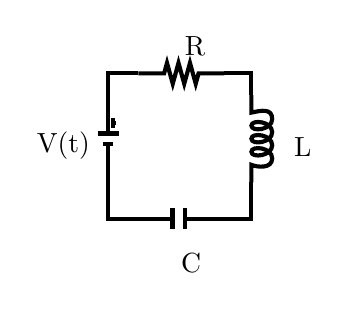
\begin{tikzpicture}
\pgftransformxscale{0.500000}
\pgftransformyscale{-0.500000}
\definecolor{dialinecolor}{rgb}{0.000000, 0.000000, 0.000000}
\pgfsetstrokecolor{dialinecolor}
\definecolor{dialinecolor}{rgb}{1.000000, 1.000000, 1.000000}
\pgfsetfillcolor{dialinecolor}
\pgfsetlinewidth{0.100000\du}
\pgfsetdash{}{0pt}
\pgfsetdash{}{0pt}
\pgfsetbuttcap
\pgfsetmiterjoin
\pgfsetlinewidth{0.100000\du}
\pgfsetbuttcap
\pgfsetmiterjoin
\pgfsetdash{}{0pt}
\definecolor{dialinecolor}{rgb}{0.000000, 0.000000, 0.000000}
\pgfsetstrokecolor{dialinecolor}
\draw (2.900000\du,9.550000\du)--(2.900000\du,10.800000\du);
\pgfsetbuttcap
\pgfsetmiterjoin
\pgfsetdash{}{0pt}
\definecolor{dialinecolor}{rgb}{0.000000, 0.000000, 0.000000}
\pgfsetstrokecolor{dialinecolor}
\draw (2.400000\du,10.800000\du)--(3.400000\du,10.800000\du);
\pgfsetbuttcap
\pgfsetmiterjoin
\pgfsetdash{}{0pt}
\definecolor{dialinecolor}{rgb}{0.000000, 0.000000, 0.000000}
\pgfsetstrokecolor{dialinecolor}
\draw (2.650000\du,11.300000\du)--(3.150000\du,11.300000\du);
\pgfsetbuttcap
\pgfsetmiterjoin
\pgfsetdash{}{0pt}
\definecolor{dialinecolor}{rgb}{0.000000, 0.000000, 0.000000}
\pgfsetstrokecolor{dialinecolor}
\draw (3.150000\du,10.050000\du)--(3.150000\du,10.550000\du);
\pgfsetbuttcap
\pgfsetmiterjoin
\pgfsetdash{}{0pt}
\definecolor{dialinecolor}{rgb}{0.000000, 0.000000, 0.000000}
\pgfsetstrokecolor{dialinecolor}
\draw (3.025000\du,10.300000\du)--(3.275000\du,10.300000\du);
\pgfsetbuttcap
\pgfsetmiterjoin
\pgfsetdash{}{0pt}
\definecolor{dialinecolor}{rgb}{0.000000, 0.000000, 0.000000}
\pgfsetstrokecolor{dialinecolor}
\draw (2.900000\du,11.300000\du)--(2.900000\du,12.550000\du);
\pgfsetlinewidth{0.100000\du}
\pgfsetdash{}{0pt}
\pgfsetdash{}{0pt}
\pgfsetbuttcap
\pgfsetmiterjoin
\pgfsetlinewidth{0.100000\du}
\pgfsetbuttcap
\pgfsetmiterjoin
\pgfsetdash{}{0pt}
\definecolor{dialinecolor}{rgb}{0.000000, 0.000000, 0.000000}
\pgfsetstrokecolor{dialinecolor}
\draw (4.350000\du,7.900000\du)--(5.595000\du,7.900000\du)--(5.733333\du,7.400000\du)--(6.010000\du,8.400000\du)--(6.286667\du,7.400000\du)--(6.563333\du,8.400000\du)--(6.840000\du,7.400000\du)--(7.116667\du,8.400000\du)--(7.255000\du,7.900000\du)--(8.500000\du,7.900000\du);
\pgfsetlinewidth{0.100000\du}
\pgfsetdash{}{0pt}
\pgfsetdash{}{0pt}
\pgfsetbuttcap
\pgfsetmiterjoin
\pgfsetlinewidth{0.100000\du}
\pgfsetbuttcap
\pgfsetmiterjoin
\pgfsetdash{}{0pt}
\definecolor{dialinecolor}{rgb}{0.000000, 0.000000, 0.000000}
\pgfsetstrokecolor{dialinecolor}
\pgfpathmoveto{\pgfpoint{9.800000\du}{8.950000\du}}
\pgfpathlineto{\pgfpoint{9.800000\du}{9.790000\du}}
\pgfpathcurveto{\pgfpoint{10.300000\du}{9.685000\du}}{\pgfpoint{10.800000\du}{9.580000\du}}{\pgfpoint{10.800000\du}{10.105000\du}}
\pgfpathcurveto{\pgfpoint{10.800000\du}{10.630000\du}}{\pgfpoint{9.800000\du}{10.735000\du}}{\pgfpoint{9.800000\du}{10.420000\du}}
\pgfpathcurveto{\pgfpoint{9.800000\du}{10.105000\du}}{\pgfpoint{10.800000\du}{10.210000\du}}{\pgfpoint{10.800000\du}{10.735000\du}}
\pgfpathcurveto{\pgfpoint{10.800000\du}{11.260000\du}}{\pgfpoint{9.800000\du}{11.365000\du}}{\pgfpoint{9.800000\du}{11.050000\du}}
\pgfpathcurveto{\pgfpoint{9.800000\du}{10.735000\du}}{\pgfpoint{10.800000\du}{10.840000\du}}{\pgfpoint{10.800000\du}{11.365000\du}}
\pgfpathcurveto{\pgfpoint{10.800000\du}{11.890000\du}}{\pgfpoint{9.800000\du}{11.995000\du}}{\pgfpoint{9.800000\du}{11.680000\du}}
\pgfpathcurveto{\pgfpoint{9.800000\du}{11.365000\du}}{\pgfpoint{10.800000\du}{11.470000\du}}{\pgfpoint{10.800000\du}{11.995000\du}}
\pgfpathcurveto{\pgfpoint{10.800000\du}{12.520000\du}}{\pgfpoint{10.050000\du}{12.415000\du}}{\pgfpoint{9.800000\du}{12.310000\du}}
\pgfpathlineto{\pgfpoint{9.800000\du}{13.150000\du}}
\pgfusepath{stroke}
\pgfsetlinewidth{0.100000\du}
\pgfsetdash{}{0pt}
\pgfsetdash{}{0pt}
\pgfsetbuttcap
\pgfsetmiterjoin
\pgfsetlinewidth{0.100000\du}
\pgfsetbuttcap
\pgfsetmiterjoin
\pgfsetdash{}{0pt}
\definecolor{dialinecolor}{rgb}{0.000000, 0.000000, 0.000000}
\pgfsetstrokecolor{dialinecolor}
\draw (4.800000\du,14.900000\du)--(6.000000\du,14.900000\du);
\pgfsetbuttcap
\pgfsetmiterjoin
\pgfsetdash{}{0pt}
\definecolor{dialinecolor}{rgb}{0.000000, 0.000000, 0.000000}
\pgfsetstrokecolor{dialinecolor}
\draw (6.000000\du,14.400000\du)--(6.000000\du,15.400000\du);
\pgfsetbuttcap
\pgfsetmiterjoin
\pgfsetdash{}{0pt}
\definecolor{dialinecolor}{rgb}{0.000000, 0.000000, 0.000000}
\pgfsetstrokecolor{dialinecolor}
\draw (6.600000\du,14.400000\du)--(6.600000\du,15.400000\du);
\pgfsetbuttcap
\pgfsetmiterjoin
\pgfsetdash{}{0pt}
\definecolor{dialinecolor}{rgb}{0.000000, 0.000000, 0.000000}
\pgfsetstrokecolor{dialinecolor}
\draw (6.600000\du,14.900000\du)--(7.800000\du,14.900000\du);
\pgfsetlinewidth{0.100000\du}
\pgfsetdash{}{0pt}
\pgfsetdash{}{0pt}
\pgfsetmiterjoin
\pgfsetbuttcap
{
\definecolor{dialinecolor}{rgb}{0.000000, 0.000000, 0.000000}
\pgfsetfillcolor{dialinecolor}
% was here!!!
{\pgfsetcornersarced{\pgfpoint{0.000000\du}{0.000000\du}}\definecolor{dialinecolor}{rgb}{0.000000, 0.000000, 0.000000}
\pgfsetstrokecolor{dialinecolor}
\draw (8.500000\du,7.900000\du)--(9.800000\du,7.900000\du)--(9.800000\du,8.950000\du);
}}
\pgfsetlinewidth{0.100000\du}
\pgfsetdash{}{0pt}
\pgfsetdash{}{0pt}
\pgfsetmiterjoin
\pgfsetbuttcap
{
\definecolor{dialinecolor}{rgb}{0.000000, 0.000000, 0.000000}
\pgfsetfillcolor{dialinecolor}
% was here!!!
{\pgfsetcornersarced{\pgfpoint{0.000000\du}{0.000000\du}}\definecolor{dialinecolor}{rgb}{0.000000, 0.000000, 0.000000}
\pgfsetstrokecolor{dialinecolor}
\draw (2.900000\du,9.550000\du)--(2.900000\du,7.900000\du)--(4.350000\du,7.900000\du);
}}
\pgfsetlinewidth{0.100000\du}
\pgfsetdash{}{0pt}
\pgfsetdash{}{0pt}
\pgfsetmiterjoin
\pgfsetbuttcap
{
\definecolor{dialinecolor}{rgb}{0.000000, 0.000000, 0.000000}
\pgfsetfillcolor{dialinecolor}
% was here!!!
{\pgfsetcornersarced{\pgfpoint{0.000000\du}{0.000000\du}}\definecolor{dialinecolor}{rgb}{0.000000, 0.000000, 0.000000}
\pgfsetstrokecolor{dialinecolor}
\draw (9.800000\du,13.150000\du)--(9.800000\du,13.150000\du)--(9.800000\du,14.900000\du)--(7.800000\du,14.900000\du);
}}
\pgfsetlinewidth{0.100000\du}
\pgfsetdash{}{0pt}
\pgfsetdash{}{0pt}
\pgfsetmiterjoin
\pgfsetbuttcap
{
\definecolor{dialinecolor}{rgb}{0.000000, 0.000000, 0.000000}
\pgfsetfillcolor{dialinecolor}
% was here!!!
{\pgfsetcornersarced{\pgfpoint{0.000000\du}{0.000000\du}}\definecolor{dialinecolor}{rgb}{0.000000, 0.000000, 0.000000}
\pgfsetstrokecolor{dialinecolor}
\draw (2.900000\du,12.550000\du)--(2.900000\du,14.900000\du)--(4.800000\du,14.900000\du);
}}
% setfont left to latex
\definecolor{dialinecolor}{rgb}{0.000000, 0.000000, 0.000000}
\pgfsetstrokecolor{dialinecolor}
\node[anchor=west] at (6.050000\du,6.600000\du){R};
% setfont left to latex
\definecolor{dialinecolor}{rgb}{0.000000, 0.000000, 0.000000}
\pgfsetstrokecolor{dialinecolor}
\node[anchor=west] at (5.865000\du,17.055000\du){C};
% setfont left to latex
\definecolor{dialinecolor}{rgb}{0.000000, 0.000000, 0.000000}
\pgfsetstrokecolor{dialinecolor}
\node[anchor=west] at (-1.080000\du,11.360000\du){V(t)};
% setfont left to latex
\definecolor{dialinecolor}{rgb}{0.000000, 0.000000, 0.000000}
\pgfsetstrokecolor{dialinecolor}
\node[anchor=west] at (7.450000\du,16.200000\du){};
% setfont left to latex
\definecolor{dialinecolor}{rgb}{0.000000, 0.000000, 0.000000}
\pgfsetstrokecolor{dialinecolor}
\node[anchor=west] at (11.315000\du,11.455000\du){L};
\end{tikzpicture}
